\documentclass{beamer}
\usepackage{mathpartir, stmaryrd}
\usepackage{wasysym}
\usepackage[normalem]{ulem}
\usepackage{listings}
\usepackage{multicol}
\usepackage{microtype}
\usepackage{color}
\usepackage{listings}

\usefonttheme[onlymath]{serif}
\definecolor{JadeGreen}{RGB}{0,168,107}
\definecolor{MunsellPurple}{RGB}{159,0,197}

\definecolor{CobaltBlue}{RGB}{0,71,171}
\definecolor{FireBrick}{RGB}{228,34,23}
\definecolor{Alabaster}{RGB}{250,250,250}

\definecolor{PaleGray}{gray}{0.93}

\setbeamertemplate{navigation symbols}{}
\setbeamertemplate{headline}{}
\setbeamercolor{example text}{fg=CobaltBlue}
\setbeamertemplate{itemize items}{$\bullet$}
\setbeamercolor{alert text}{fg=FireBrick}

\lstset{language=ML,
        columns=fullflexible,
        keepspaces=true,
        basicstyle=\ttfamily,
        tabsize=4,
        keywordstyle={\color{CobaltBlue}},
        morekeywords={,dcl,set,get,cmd,return,}
        escapeinside={"*}{*"},
        moredelim=*[is][\color{FireBrick}]{`}{'},
        literate={->}{{$\shortrightarrow$}}1
                 {->}{{$\gets$}}1
                 {\\}{{$\lambda$}}1
                 {times}{{$\times$}}1
                 {alpha}{{$\alpha$}}1
                 {beta}{{$\beta$}}1
                 {gamma}{{$\gamma$}}1
                 {vdots}{{\vdots}}1}

% Formatting tools
\newcommand{\declareJudgement}[1]{\framebox{$\displaystyle{}{#1}$}}
\newcommand{\different}[1]{{\color{red} #1}}

% Categories stuff
\newcommand{\Ccat}{\ensuremath{\mathbb{C}}}
\newcommand{\Dcat}{\ensuremath{\mathbb{D}}}
\newcommand{\op}[1]{\ensuremath{#1^{\mathsf{op}}}}
\newcommand{\SET}{\ensuremath{\mathbf{Set}}}
\newcommand{\DCPO}{\ensuremath{\mathbf{Dcpo}}}
\newcommand{\presheaves}[1]{\ensuremath{\widehat{#1}}}
\newcommand{\transpose}[1]{\ensuremath{\widehat{#1}}}
\newcommand{\pair}[2]{\ensuremath{\left\langle #1, #2 \right\rangle}}
\newcommand{\univ}{\ensuremath{\mathcal{U}}}
\newcommand{\mono}{\ensuremath{\rightarrowtail}}
\newcommand{\yoneda}{\ensuremath{\mathsf{y}}}

% Math stuffs
\newcommand{\upred}[1]{\ensuremath{\mathsf{UPred}(#1)}}
\newcommand{\reach}{\ensuremath{\mathrel{\sqsubseteq}}}
\newcommand{\breach}{\ensuremath{\mathrel{\sqsupseteq}}}
\newcommand{\mto}{\ensuremath{\xrightarrow{\mathsf{mon}}}}
\newcommand{\pto}{\ensuremath{\rightharpoonup}}
\newcommand{\pow}[1]{\ensuremath{\mathcal{P}(#1)}}
\newcommand{\powfin}[1]{\ensuremath{\mathcal{P_{\mathrm{fin}}}(#1)}}
\newcommand{\card}[1]{\ensuremath{\left\vert #1 \right\vert}}
\newcommand{\real}{\ensuremath{\mathbb{R}}}
\newcommand{\nat}{\ensuremath{\mathbb{N}}}
\newcommand{\cbult}{\ensuremath{\mathrm{CBUlt}}}
\newcommand{\cle}{\ensuremath{\lesssim}}
\newcommand{\ceq}{\ensuremath{\cong}}
\newcommand{\relR}{\ensuremath{\mathrel{\mathcal{R}}}}
\newcommand{\relS}{\ensuremath{\mathrel{\mathcal{S}}}}
\newcommand{\AND}{\ensuremath{\mathrel{\wedge}}}
\newcommand{\OR}{\ensuremath{\mathrel{\vee}}}
\newcommand{\den}[1]{\ensuremath{\llbracket #1 \rrbracket}}
\newcommand{\definitely}[1]{\ensuremath{\lceil #1 \rceil}}
\newcommand{\possibly}[1]{\ensuremath{\lfloor #1 \rfloor}}
\newcommand{\defs}{\ensuremath{\mathrel{\triangleq}}}
\newcommand{\bifix}{\ensuremath{\mathsf{bifix}}}
\newcommand{\disjoint}{\ensuremath{\mathop{\#}}}
\newcommand{\hole}{\ensuremath{\square}}
\newcommand{\sincl}[1]{\ensuremath{\mathsf{succ}(#1)}}
\newcommand{\join}{\ensuremath{\bigvee}}
\newcommand{\cless}{\ensuremath{\lessapprox}}
\newcommand{\aless}{\ensuremath{\lesssim}}

\DeclareMathOperator{\dom}{Dom}

% Sets
\newcommand{\states}{\ensuremath{\mathrm{State}}}
\newcommand{\worlds}{\ensuremath{\mathbb{W}}}
\newcommand{\assignables}{\ensuremath{\mathrm{Assignable}}}
\newcommand{\nrel}[1]{\ensuremath{\mathbb{R}_{#1}}}
\newcommand{\semtypes}{\ensuremath{\mathbb{T}}}
\newcommand{\types}{\ensuremath{\mathrm{Type}}}
\newcommand{\typesEnv}{\ensuremath{\mathrm{TypeEnv}}}
\newcommand{\term}{\ensuremath{\mathrm{Term}}}
\newcommand{\urel}{\ensuremath{\mathrm{URel}}}

% judgments
\newcommand{\guardJ}[2]{\ensuremath{\text{$#1.\,#2$\ \textsf{guarded}}}}
\newcommand{\hasE}[2]{\ensuremath{#1 \mathrel{:} #2}}
\newcommand{\hasM}[2]{\ensuremath{#1 \mathrel{\div} #2}}
\newcommand{\hasKJ}[2]{\ensuremath{#1 \vdash \hasE{#2}{\mathrm{\kind}}}}
\newcommand{\hasTJ}[4]{\ifthenelse{\isempty{#1}}%
  {\ensuremath{#2 \vdash \hasE{#3}{#4}}}%
  {\ensuremath{#1;#2 \vdash \hasE{#3}{#4}}}}
\newcommand{\hasEJ}[5]{\ifthenelse{\isempty{#1}}%
  {\ensuremath{#2; #3 \vdash \hasE{#4}{#5}}}%
  {\ensuremath{#1; #2; #3 \vdash \hasE{#4}{#5}}}}
\newcommand{\hasESigJ}[5]{\ensuremath{#1; #2 \vdash_{#3} \hasE{#4}{#5}}}
\newcommand{\hasMJ}[5]{\ensuremath{#1; #2 \vdash_{#3} \hasM{#4}{#5}}}
\newcommand{\hasCEJ}[9]{\ensuremath{#5 : (#1; #2 \vdash_{#3} #4) \rightsquigarrow (#6; #7 \vdash_{#8} #9)}}

\newcommand{\subKJ}[3]{\ifthenelse{\isempty{#1}}%
{\ensuremath{{#2} \leq {#3}}}%
{\ensuremath{{#1} \vdash {#2} \leq {#3}}}}

\newcommand{\equivESigJ}[6]{\ensuremath{#1; #2 \vdash_{#3} \hasE{#4 \cong #5}{#6}}}
\newcommand{\approxESigJ}[6]{\ensuremath{#1; #2 \vdash_{#3} \hasE{#4 \aless #5}{#6}}}
\newcommand{\equivMJ}[6]{\ensuremath{#1; #2 \vdash_{#3} \hasM{#4 \cong #5}{#6}}}

\newcommand{\step}[2]{\ensuremath{#1 \mapsto #2}}
\newcommand{\steps}[2]{\ensuremath{#1 \mapsto^* #2}}
\newcommand{\stepM}[4]{\ensuremath{(#1, #2) \mapsto (#3, #4)}}
\newcommand{\stepsM}[5][*]{\ensuremath{(#2, #3) \mapsto^{#1} (#4, #5)}}

\newcommand{\dec}[4][i]{\ensuremath{#2 \rhd^{#1} #3 : #4}}
\newcommand{\valueJ}[1]{\ensuremath{#1\ \mathsf{value}}}
\newcommand{\finalJ}[2]{\ensuremath{(#1, #2)\ \mathsf{final}}}

% language
\newcommand{\kind}{\ensuremath{\mathsf{kind}}}
\newcommand{\later}{\ensuremath{{\blacktriangleright}}}
\newcommand{\ilater}{\ensuremath{{\triangleright}}}
\newcommand{\rec}[2]{\ensuremath{\mu #1.\, #2}}
\newcommand{\fn}[2]{\ensuremath{#1 \to #2}}
\newcommand{\tp}{\ensuremath{\mathsf{T}}}
\newcommand{\unit}{\ensuremath{\mathsf{unit}}}
\newcommand{\cmd}[1]{\ensuremath{\mathsf{cmd}(#1)}}

\newcommand{\ap}[2]{\ensuremath{#1\ #2}}
\newcommand{\lam}[3]{\ensuremath{\lambda #1 {:} #2.\, #3}}
\newcommand{\into}[1]{\ifthenelse{\isempty{#1}}%
  {\ensuremath{\mathsf{in}}}%
  {\ensuremath{\mathsf{in}\,#1}}}
\newcommand{\out}[1]{\ifthenelse{\isempty{#1}}%
  {\ensuremath{\mathsf{out}}}%
  {\ensuremath{\mathsf{out}\,#1}}}
\newcommand{\delay}{\mathsf{next}}
\newcommand{\fix}{\mathsf{fix}}
\newcommand{\letdelay}[3]{\ensuremath{\mathsf{let\ next\ } #1 = #2 \mathsf{\ in\ } #3}}
\newcommand{\all}[3]{\ensuremath{\forall #1 {:} #2.\, #3}}
\newcommand{\allNoKind}[2]{\ensuremath{\forall #1.\, #2}}

\newcommand{\Ap}[2]{\ensuremath{#1[#2]}}
\newcommand{\Lam}[3]{\ensuremath{\Lambda #1 {:} #2.\, #3}}

\newcommand{\LamNoKind}[2]{\ensuremath{\Lambda #1.\, #2}}
\newcommand{\ret}[1]{\ensuremath{\mathsf{ret}(#1)}}
\newcommand{\get}[1]{\ensuremath{\mathsf{get}[#1]}}
\newcommand{\set}[2]{\ensuremath{\mathsf{set}[#1](#2)}}
\newcommand{\dcl}[3]{\ensuremath{\mathsf{dcl}\ #1 := #2\ \mathsf{in}\ #3}}
\newcommand{\bnd}[3]{\ensuremath{\mathsf{bnd}\ #1 \gets #2;\ #3}}

\newcommand{\trunc}{\ensuremath{\mathsf{trunc}}}

\newcommand{\littrue}{\ensuremath{\mathsf{true}}}
\newcommand{\litfalse}{\ensuremath{\mathsf{false}}}

\newcommand{\zap}{\ensuremath{\circledast}}

\title{The Next 700 Failed \\Step-Index-Free Logical Relations}
\author{Daniel Gratzer}
\date{\today}

\begin{document}
\begin{frame}
  \titlepage
\end{frame}

\begin{frame}
  \centering
  Goals for today's talk:
  \begin{itemize}
  \item Explain the title.
  \item Maybe answer questions.
  \end{itemize}
\end{frame}

\begin{frame}
  \begin{center}
    \bf When are two programs \alert<5>{equal}?
  \end{center}
  \begin{enumerate}
  \item<2-> Checking compiler optimizations
  \item<3-> Formalize data abstraction
  \item<4-> Compositional verification proofs
  \end{enumerate}
\end{frame}

\begin{frame}
  \begin{center}
    \bf What should equality mean?
  \end{center}
  \pause
  \begin{itemize}
  \item Should equality be decidable?
    \pause
  \item Should equality consider computational time?
    \pause
  \item Should free variables be treated as \emph{indeterminates}?
  \end{itemize}
\end{frame}

\begin{frame}
  \begin{center}
    Two programs are equal if you can replace one with another in a
    bigger program without causing the bigger program to diverge.
  \end{center}
\end{frame}

\begin{frame}
  \centering
  To prove that two programs, $e_1$ and $e_2$ are equal...
  \begin{enumerate}
  \item Pick a program with a hole in it, $C$
  \item Test whether $C[e_1]$ terminates
  \item Test whether $C[e_2]$ terminates
  \item If the results disagree, they're not equal
    \pause
  \item Rinse and repeat for every possible $C$
  \end{enumerate}
\end{frame}

\begin{frame}
  Contextual equivalence has some advantages:
  \begin{itemize}
  \item Easily scales to different languages
  \item \emph{Extensional}
  \item Allows us to replace equals by equals
  \end{itemize}
\end{frame}

\begin{frame}
  \begin{center}
    \it Rinse and repeat for every possible $C$
  \end{center}
  \pause
  There are a lot of $C$s.
  \pause
  It's not obvious how to write a proof which handles all of them.
\end{frame}

\begin{frame}
  \centering
  Key idea: use {\color<2>{PaleGray} the structure of the} types
  {\color<2>{PaleGray} to classify what contexts are worth considering.}
  \pause
  \bigskip

  \begin{figure}
    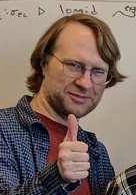
\includegraphics[height=5cm,keepaspectratio]{happy-karl}
  \end{figure}
\end{frame}

\begin{frame}
  \centering
  An example: functions
  \pause
  \bigskip
  \begin{align*}
    f_1 \sim f_2 &: \fn{\tau_1}{\tau_2} \triangleq \forall a_1, a_2.\\
    &a_1 \sim a_2 : \tau_1 \implies \ap{f_1}{a_1} \sim \ap{f_2}{a_2} : \tau_2
  \end{align*}
\end{frame}

\begin{frame}
  This works well for ``logical'' connectives: $\to$, $\times$, $+$,
  $\exists$, $\forall$...
  \pause

  What about types that are not so obviously logical?
\end{frame}

\begin{frame}
  \centering
  This works well for ``logical'' connectives: $\to$, $\times$, $+$,
  $\exists$, $\forall$...
\end{frame}

\begin{frame}
  \centering
  What about state?

  \pause
  \bigskip

  We consider a language with a type classifying imperative
  computation: $\cmd{\tau}$.
\end{frame}

\begin{frame}[fragile]
  \centering
  \begin{minipage}{0.5\textwidth}
    \centering
\begin{lstlisting}
cmd(
  dcl alpha := 1 in
  return cmd(get alpha)
)
\end{lstlisting}
  \end{minipage}%
  \begin{minipage}{0.5\textwidth}
    \centering
\begin{lstlisting}
cmd(cmd(return 1))
\end{lstlisting}
  \end{minipage}
\end{frame}

\begin{frame}
  \centering
  How do we define $\cmd{m_1} \sim \cmd{m_2} : \cmd{\tau}$?
  \pause
  \bigskip
  \begin{itemize}
  \item Commands are functions: heap to heap and a result
  \item $\sim$ for commands should be like $\sim$ for functions
  \item When are two heaps related?
  \end{itemize}
\end{frame}

\begin{frame}
  \begin{quote}\centering
    \bf\it When are two heaps related?
  \end{quote}

  \begin{itemize}
  \item Simplest answer is that they're related pointwise\\
    \[
      h_1 \sim h_2 : \Sigma \defs
      \forall \alpha : \tau \in \Sigma.\ h_1(\alpha) \relR h_2(\alpha) : \tau
    \]
  \item What equality should be used at each point? (What is $\relR$)
  \end{itemize}
\end{frame}

\begin{frame}
  \centering
  There are 3 reasonable choices for $\relR$:
  \begin{enumerate}
  \item $\relR$ could be stricter than $\sim$
  \item $\relR$ could be exactly $\sim$
  \item $\relR$ could be weaker than $\sim$
  \end{enumerate}
  \pause
  \bigskip

  All of these are bad ideas.
  \pause
  \bigskip
  \begin{enumerate}
  \item $\sim$ will not be reflexive
  \item $\sim$ will not be well-defined
  \item $\sim$ will not be reflexive
  \end{enumerate}
\end{frame}

\begin{frame}
  \centering
  \begin{quote}
    \bf\it $\relR$ could be exactly $\sim$: $\sim$ will not be well-defined
  \end{quote}
  Alternative idea: parameterize $\sim$ by a \emph{world} telling us
  how to compare.
\end{frame}

\begin{frame}
  \centering
  Kripke Logical relations
  \begin{itemize}
  \item Parameterize $\sim$ by a partial order $\worlds$
  \item $w \in \worlds$ is a relation on heaps
  \item $w_1 \le w_2$ if $w_2$ relates extensions of heaps related by
    $w_1$
  \item $\sim$ is monotone
  \end{itemize}
  \bigskip
  \[
    h_1 \sim h_2 : w \defs \forall \alpha \in \Dom(w).\ (h_1(\alpha), h_2(\alpha)) \in w(\alpha)
  \]
\end{frame}

\begin{frame}
  \centering What should $\worlds$ be?
  \begin{align*}
    \semtypes &= \worlds \mto \pow{\term \times \term}\\
    \worlds &= \assignables \pto \semtypes
  \end{align*}
  \pause
  \bigskip
  No solutions in sets.
\end{frame}

\begin{frame}
  Step-indexing: solve these equations up to $n$ unfoldings.

  \begin{itemize}
  \item $\sim$ can now means that two programs are equal for at least
    $n$ steps
  \item Can't get rid of these steps
  \end{itemize}
\end{frame}

\begin{frame}
  \centering
  Idea of this thesis: can we solve these equations in a different
  way?

  \pause
  \bigskip

  No.
\end{frame}
\end{document}
